\documentclass[withoutpreface,bwprint]{cumcmthesis}
%\usepackage{subfigure}
\title{存算一体技术}
\author{2021113140符世博}
\date{}
\begin{document}
\maketitle

\section{存算一体技术背景及发展历程}
\subsection{存算一体技术背景}

\subsubsection{“冯$\cdot$诺伊曼瓶颈”问题}
在冯·诺依曼架构中,数据首先从存储器中获取到处理器进行处理,然后再写回存储器。由于计算核心和存储器之间的有限带宽限制了数据交换的速度,这导致了计算核心处理速度和存储器访问速度之间的差异,进一步减缓了处理速度,即所谓的“冯·诺依曼瓶颈”。

此外,存储器数据访问速度远低于中央处理器的数据处理速度,也被称为“存储墙”问题。数据搬运的能耗比浮点计算高出1-2个数量级,而芯片内一级缓存的功耗达到25$pJ/bit$,动态随机存取内存访问功耗为1.3-2.6$nJ/bit$,是芯片内缓存功耗的倍,进一步增加了数据访问能耗,即“功耗墙”问题。

随着摩尔定律的放缓和工艺尺寸微缩变得越来越困难,传统架构提升使性能增长速度也在变缓,人们试图寻找一种新的计算范式来取代现有计算范式以跳出冯·诺依曼架构和摩尔定律的围墙,并进行多种路径尝试。


\subsubsection{高算力需求的挑战}
当前,随着人工智能等领域的迅速发展,对算力的需求呈现出快速增长的趋势,而与之形成鲜明对比的是算力提升的速度放缓。以人工智能为例,从1960年到2010年,算力需求每两年提升一倍,但自从2012年Alexnet开始使用图形处理器进行训练以来,算力的提升速度进一步加快,每3-4个月就会提升一倍。举例来说,谷歌AlphaGo在与李世石对弈中仅需使用1920个CPU和280个GPU;而谷歌GPT-3开源人工智能模型拥有1746亿个参数,据估算,训练这个模型需要3000-5000块英伟达A100GPU,并且GPT-3.5的训练显卡数量更进一步增至2万块。这种急剧增长的算力需求与算力提升放缓之间的矛盾日益显现。


\subsection{存算一体技术解决方案}

\subsubsection{高带宽数据通信}
高带宽数据通信主要涉及光互联技术和2.5D/3D堆叠技术。光互联技术具有高带宽、长距离、低损耗、无串扰和电磁兼容等优势,但是在芯片内部难以实现光互联器件,光交换重新连接开销和延迟较大,且实用化成本高,难以大规模应用。另一方面,2.5D/3D堆叠技术通过增大并行带宽或利用串行传输提升存储带宽,简化系统存储控制设计难度,具有高集成度、高带宽和高能效等性能优势。然而,目前2.5D/3D堆叠技术仅对分立器件或芯片内部进行优化设计,“存”和“算”本质上仍然是分离的,难以填补“存—算”之间的鸿沟。

\subsubsection{缓解访存延迟和功耗的内存计算}
为了弥合“存—算”之间的巨大鸿沟,内存计算的概念应运而生。内存计算主要包括两种技术类型。一种是横向扩展,主要是指分布式内存计算,其典型代表是Spark架构,这是一种软件方案。另一种是纵向扩展,又可以分为两种:一种是近数据端处理,包括近存储计算和近内存计算;另一种是存算一体,它依赖于经典存储器件或者新型的存算器件,如\cref{fig:1}所示。

\begin{figure}[H]
    \centering
    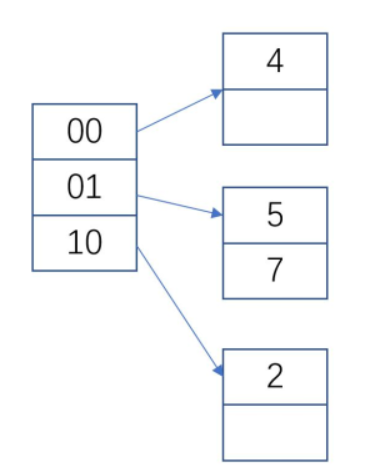
\includegraphics[width=0.95\textwidth]{1}
    \caption{内存计算体系}
    \label{fig:1}
\end{figure}

\section{忆阻器存算一体技术}

忆阻器是一种新型纳米器件,阻值与流经的
电荷相关且具有非易失性。忆阻器研究涉及微电
子、材料学、凝聚态物理、人工智能等学科领域,
应用涵盖信息存储、非易失逻辑、非线性动
力学、混沌电路、忆阻神经网络、神经
元模型等众多方向,并由此实现仿生神经元、
长短期记忆、联想学习等认知功能。此外,凭借高
密度、低延迟、非易失性等特性,忆阻器成为存算
一体技术的重要研究方向,同时也为感存算一体技
术提供了可靠的解决方案。

忆阻器存算一体技术常以大规模交叉阵列为
基础,参加计算的电导直接存储在阵列中。随着半
导体工艺的快速发展,纳米传感器同忆阻器集成,
感知、存储和运算进一步融合,传感器感知的模拟
信号直接经过忆阻器阵列运算和存储,减少数据
交换。

\subsection{存算一体的逻辑电路}
存算一体逻辑电路包含忆阻器实质蕴含逻辑(material IMPlication logic, IMP)和忆阻器辅助逻
辑(Memristor-Aided loGIC, MAGIC),以电阻
状态为参量,基于阻值转变实现逻辑运算并将结果
直接存储为阻值。

如\cref{fig:2.1}所示,两个并联的忆阻器串联接地电
阻构成基本IMP逻辑单元。Vset是忆阻器置逻辑1的
负电压,Vclear是忆阻器置逻辑0的正电压。Vclose是
阻值转变阈值电压,Vcond是不改变阻值的负电压。
IMP的操作步骤如下:(1)通过对忆阻器P和Q施加
Vset或者Vclear将整个逻辑单元初始化;(2)对忆阻器
P和Q的正端分别施加大小为Vcond和Vset的电压;
(3)根据电路分压原理,操作结果存储为忆阻器Q的
阻值。如\cref{fig:2.2}所示,两忆阻器正端相连构成辅助
逻辑非门。操作步骤如下:(1)将忆阻器M2设定初
始状态;(2)整体施加V0的电压(V0>Vclear>=V0/2),
结果存储为M2阻态。

\begin{figure}[H]
    \centering
    \begin{minipage}[c]{0.45\textwidth}
        \centering
        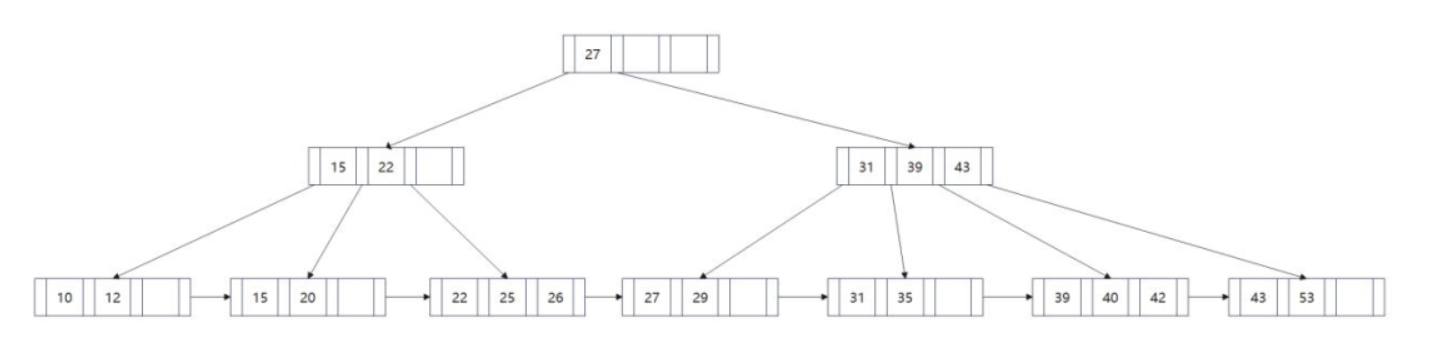
\includegraphics[width=0.95\textwidth]{2}
        \subcaption{忆阻器实质蕴含逻辑}
        \label{fig:2.1}
    \end{minipage}

    \begin{minipage}[c]{0.45\textwidth}
        \centering
        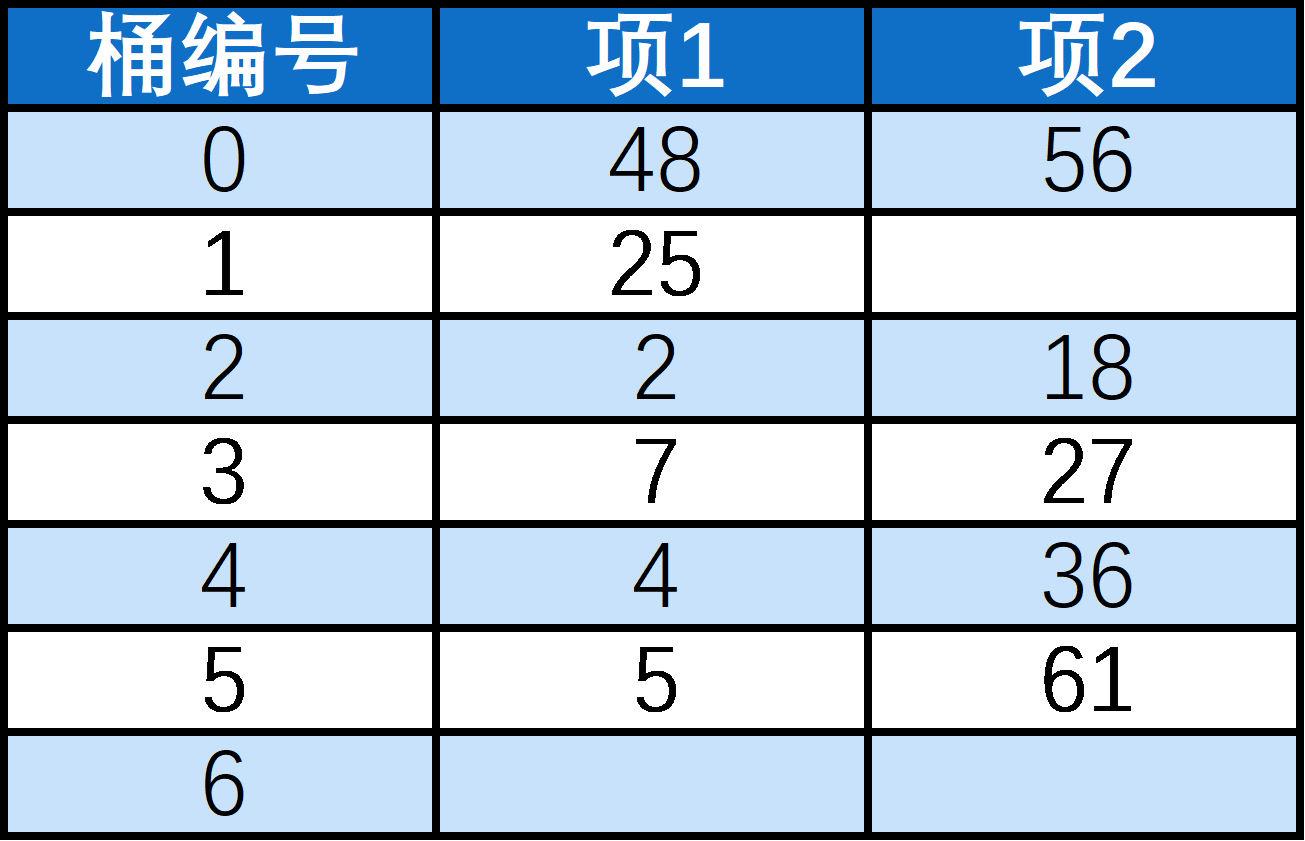
\includegraphics[width=0.95\textwidth]{3}
        \subcaption{忆阻器辅助逻辑}
        \label{fig:2.2}
    \end{minipage}
    \caption{基于忆阻器的逻辑单元}
    \label{fig:2}
\end{figure}

\subsection{基于忆阻器的全加器}

根据IMP和MAGIC设计方法,Zahiruddin Alamgir等人研制出了基于忆阻器的全加器如\cref{fig:3}。

在这里,黑色填充的方块表示关断(高电阻)忆阻器,其他方块表示文字或其否定。输入位是$A$和$B$,进位是$C_{in}$。布尔值“$False$”或“$0$”对应于关闭的忆阻器,布尔值“$True$”或“$1$”对应于打开的忆阻器。横杆设计可以通过在底部导线上施加电压来计算$Sum$和$C_{out}$。当$Sum$为“$True$”或“$1$”时,大电流将沿第一行流过,而当$Sum$为“$False$”或“$0$”时,电流可忽略不计。类似地,当“$C_{out}$”为“$1$”时,大电流将沿着第二行流过,当“$C_{out}$”逻辑电平为“$0$”时,可忽略电流将流过。因此,如果我们在第一排和第二排的输出处添加高阻负载$R_1$和$R_2$($R_1=R_2=50kΩ$),当$Sum$为“$1$”和$C_{out}$为“$0$”时,$R1(VR1)$上的压降将远远高于$R2(VR2)$上的压降,反之亦然。当$Sum$和$C_{out}$均为“$0$”或均为“$1$”时,两个负载上的电压降分别可以忽略不计或很高。

\begin{figure}[H]
    \centering
    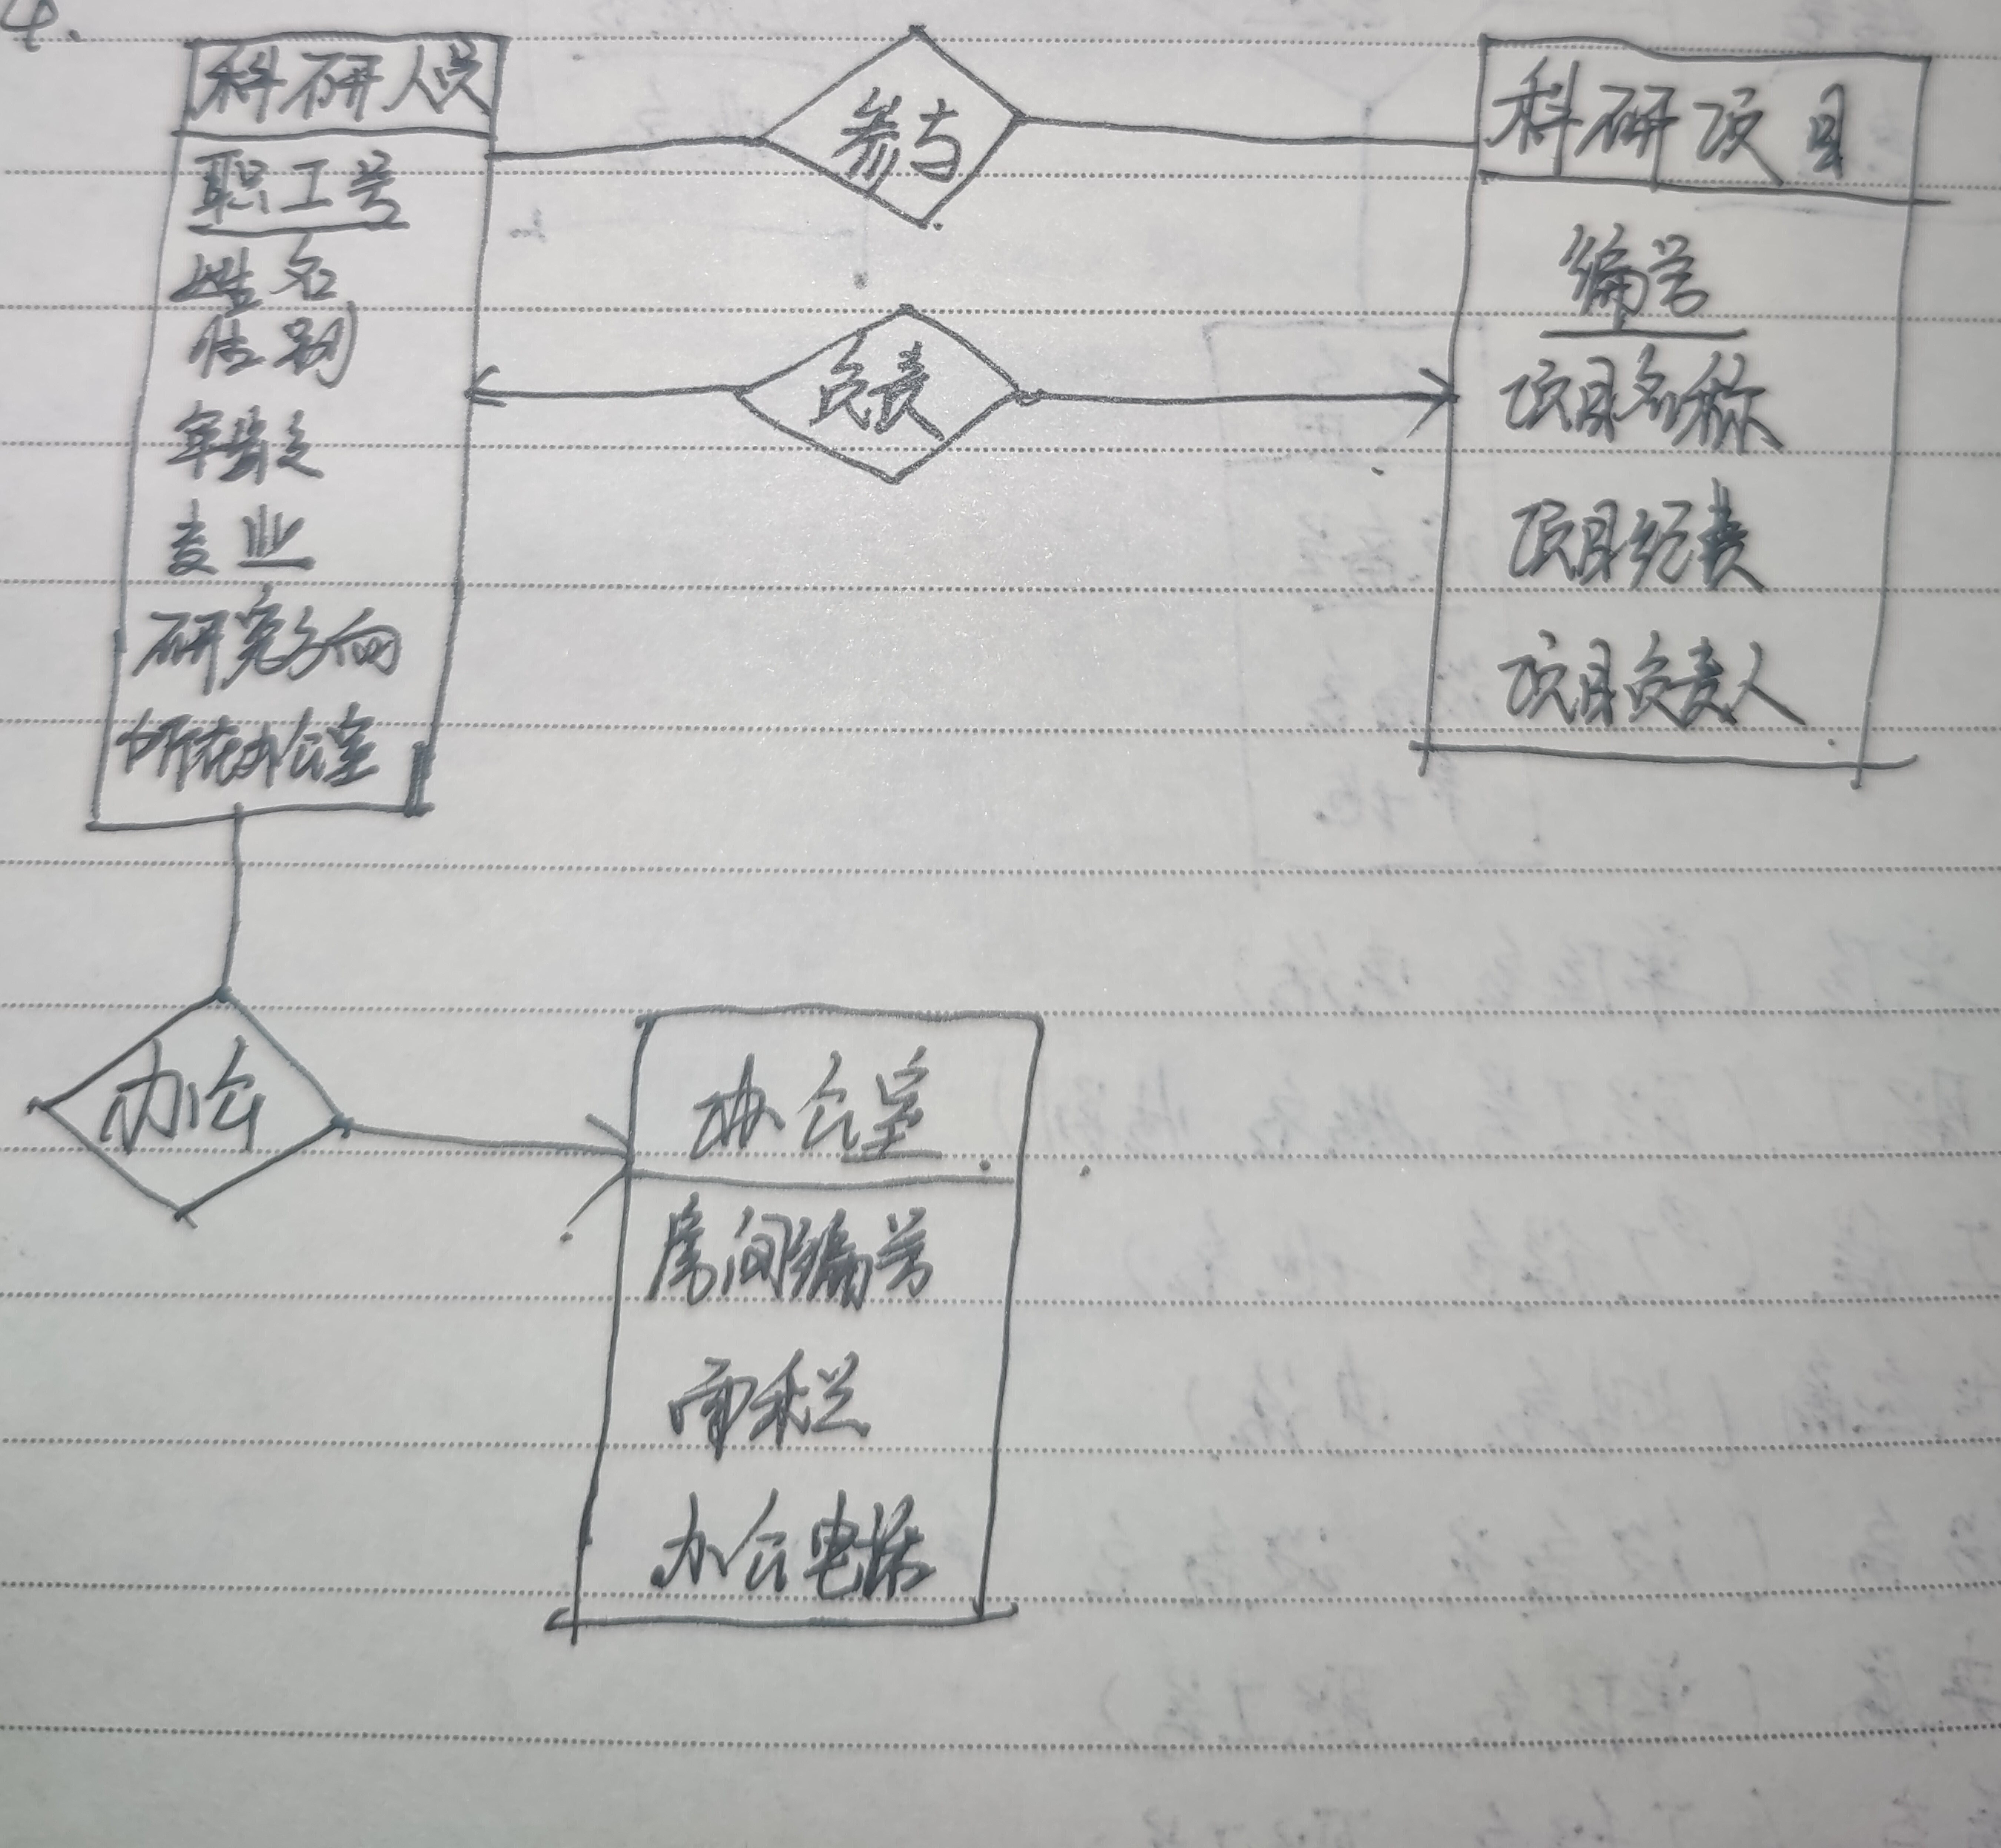
\includegraphics[width=0.95\textwidth]{4}
    \caption{基于忆阻器的全加器示意图}
    \label{fig:3}
\end{figure}

为了阐明电流如何流动以区分逻辑电平,以一个特定的示例为例,其中输入为$A=1$,$B=0$,$C_{in}=1$。每个块代表在交叉棒结处的一个忆阻器:黑框是关断的忆阻器,黄框是关断的忆阻器,根据上面解释的设计,白框是开(低阻状态)的忆阻器。在\cref{fig:3}中,虚线显示了当在底部行施加电压时的电流。在这种情况下,电流流过$C_{out}$纳米线,$R_2$上的电压降远高于$R_1$上的电压降。因此,$C_{out}$将输出高。



\section{存算一体技术挑战}
\subsection{器件特性难以满足全部需求}
存算一体技术功能器件纷繁多样,然而目前尚未有一种器件的性能能满足全部应用需求。器件存在均一性差、循环耐久性差、器件状态漂移等问题,目前已有一些优化和解决的方法,但尚未根本解决上述问题。

\subsection{阵列存在泄露路径、写串扰以及寄生电容电阻问题}

存算一体芯片网格阵列面临泄露路径、写串扰以及寄生电容电阻三大问题。在读取器件阻值时,泄露路径的存在引入了并联的电流通路,可能造成错误的读取结果。泄露路径还会带来额外的功耗,并随着阵列规模的扩大而变得更加严重。由于阵列高度并行性带来的写串扰问题会使未被选中器件的阻值受到一定影响。寄生电容、电阻会使电路延迟增加,使远端器件工作异常。

\subsection{现有集成电路设计与集成技术难以满足需求}

控制辅助电路面积和功耗占比太高,外围的器件比存算的部分大很多,外围功耗也会减少存算一体的收益。设计方面,CMOS走在前沿,与存储存在工艺差距,而统一制程将增加硬件开销,独立制程又将增加系统复杂度。3D异质集成是可行的路径。

\subsection{架构设计与开发工具有待标准化}

计算的多样性与计算定制性之间存在矛盾。不同计算网络需要定制化的存算一体架构,而全定制又不利于推广。软件和开发工具方面,缺少标准化的异构编程框架;数据映射、数据流配置缺少工具;模拟计算的“模糊/随机性”还需要进行图灵完备性的检验。

\end{document}